\documentclass{article}

% if you need to pass options to natbib, use, e.g.:
%     \PassOptionsToPackage{numbers, compress}{natbib}
% before loading neurips_2020

% ready for submission
% \usepackage{neurips_2020}

% to compile a preprint version, e.g., for submission to arXiv, add add the
% [preprint] option:
% \usepackage[preprint]{neurips_2020}

% to compile a camera-ready version, add the [final] option, e.g.:
\usepackage[final]{neurips_2020}

% to avoid loading the natbib package, add option nonatbib:
% \usepackage[nonatbib]{neurips_2020}

\usepackage[utf8]{inputenc} % allow utf-8 input
\usepackage[T1]{fontenc}    % use 8-bit T1 fonts
\usepackage{hyperref}       % hyperlinks
\usepackage{url}            % simple URL typesetting
\usepackage{booktabs}       % professional-quality tables
\usepackage{amsfonts}       % blackboard math symbols
\usepackage{nicefrac}       % compact symbols for 1/2, etc.
\usepackage{microtype}      % microtypography
\usepackage{xcolor}
\usepackage{media9}
\usepackage{float}
\usepackage{graphicx}
\usepackage{blindtext}
\usepackage{subcaption}
\usepackage{amsmath}

\title{A Transformer-Based Generative Model for Efficient and Specific CRISPR gRNA Design}

\author{
  \makebox[\linewidth]{
  \normalfont
    \begin{tabular}{ccc}
      \textbf{Tien Vu} & \textbf{Daniel Chen} & \textbf{Anton John Del Mar} \\
      Electrical and Computer Engineering & Electrical and Computer Engineering & Electrical and Computer Engineering \\
      University of California, San Diego & University of California, San Diego & University of California, San Diego \\
      \texttt{tqvu@ucsd.edu} & \texttt{dychen@ucsd.edu} & \texttt{adelmar@ucsd.edu}
    \end{tabular}
  }\\[1ex]  
}

\begin{document}

\maketitle

\iffalse
\begin{abstract}
There is a lot of potential health improvements with the development of genome editing through CRISPR-Cas9. CRISPR-Cas9 is a gene-editing tool that uses a guide RNA to direct the Cas9 enzyme to a specific DNA sequence, where it makes a precise cut to modify the gene. In this project we aim to use transformers to generate gRNA's for CRISPR-Cas9 in hopes to develop a method of creating the most effecient gRNA of a given target DNA sequence. 
\end{abstract}
\fi 

\vspace{-2em}

\section{Motivation}
CRISPR-Cas9 is a gene-editing tool that uses a guide RNA (gRNA) to direct the Cas9 enzyme to a specific DNA sequence, where it makes a precise cut to modify the gene. Predictive ranking models are oftentimes used to identify which gRNA sequence in a pre-existing pool will yield the most activity (i.e. effectiveness) at a particular DNA test site \hyperref[Reference 3]{[3]}. However, these pre-existing gRNA pools are typically obtained using rule-based heuristics and empirically validated by researchers \hyperref[Reference 4]{[4]}. Thus, the input pool may fail to capture other possible high-efficiency gRNAs that fall outside of these rules. With that said, having a model that can generate new gRNA sequences and score them can provide greater insight for researchers to determine if they already have an optimal gRNA sequence or if there are better options they can test. Our paper will investigate the possible advantages of this approach, particularly its ability to accelerate optimal gRNA discovery with scored sequences. This expands the existing search pool and helps researchers identify gRNA sequences with higher predicted activity for a given DNA target site.

\begin{figure}[H]
    \centering
    \begin{minipage}{0.32\textwidth}
        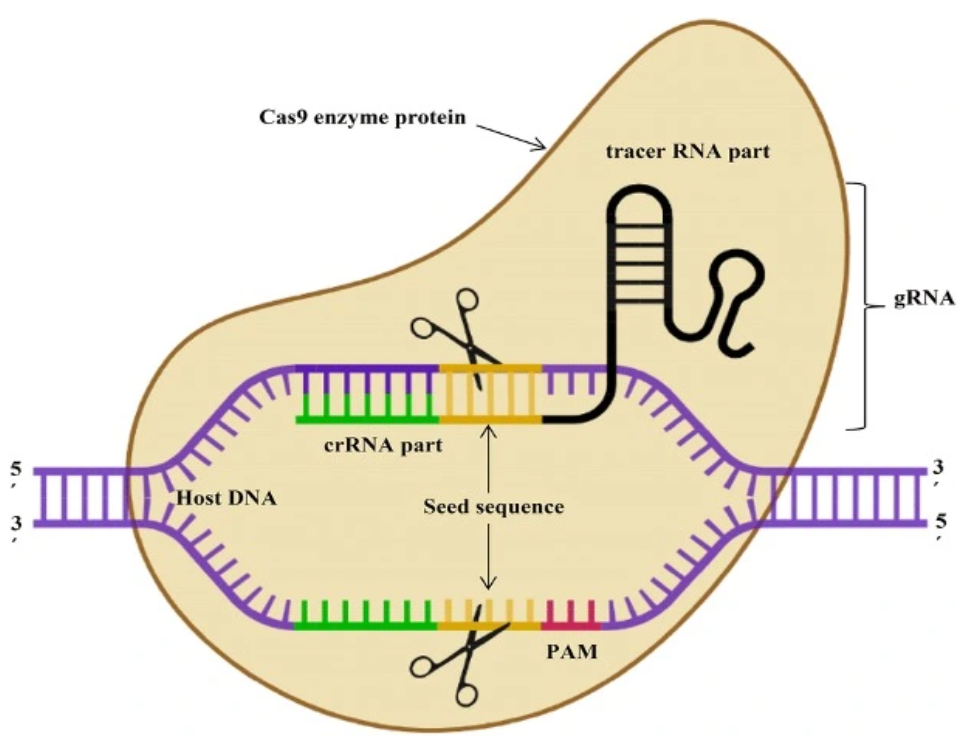
\includegraphics[width=\linewidth]{Pictures/CRISPR_Cas9.png} 
    \end{minipage}
    \caption{CRISPR-Cas9 system is a monomeric protein consisting of a single Cas9 enzyme that makes a complex with a guide RNA (gRNA) \hyperref[Reference 10]{[10]}} 
\end{figure}

\vspace{-1em}

\section{Problem}
Gene editing remains at the forefront of modern biomedical research, holding immense potential for the treatment of unique genetic disorders and complex diseases. Of these technologies, CRISPR-Cas9 is a widely-used approach that relies on gRNA to direct Cas9 enzymes to a target DNA site for precise genomic modifications \hyperref[Reference 5]{[5]}. The accuracy and effectiveness of CRISPR-Cas9 heavily depends upon the construction of the gRNA, such that it closely matches the target sequence to maximize on-target activity while minimizing off-target edits \hyperref[Reference 6]{[6]}. However, gRNA design is a non-trivial optimization problem that must balance tightly-coupled biological factors, such as PAM compatibility, sequence features, genomic location, and self-complementarity \hyperref[Reference 6]{[6]}\hyperref[Reference 8]{[8]}\hyperref[Reference 11]{[11]}. In this context, deep generative models stand out as an opportunity to synthesize optimal gRNA sequences given an input target DNA sequence.  


\section{Related Works}
Although CRISPR was first discovered in 1987, it was not until 2012 that Nobel Laureates Jennifer Doudna and Emmanuelle Charpentier discovered the use of the CRISPR-Cas9 system in precise gene editing \hyperref[Reference 5]{[5]}. Despite the relative novelty of this technology, research in improving CRISPR-Cas9 is ever expanding. This includes predictive ranking models that score existing gRNA efficiency based on a target sequence and contextual features, heuristic rule-based models that generate gRNAs without deep learning, and existing generative models that are still at their infancy. However, each of these approaches all have their limitations which we aim to address with our approach. Rankers are trained on data of gRNA that have been tested and bound to Cas9 and how well they perform at the reaching their target \hyperref[Reference 7]{[7]}. They may face biases in their ranking, favouring gRNA similar to their training set. Relative rankers are also limited to only scoring existing gRNA performance, but it cannot generate the gRNA itself and needs users to find their own sequences to test on. If a user were to generate gRNAs that are based on poor assumptions, a ranking model will still output a best performing gRNA despite all of them being from a suboptimal pool \hyperref[Reference 7]{[7]}. Existing heuristic models such as CHOPCHOP are limited by the rules researchers know for generating gRNA but may be missing features and patterns that can be learned by deep learning models \hyperref[Reference 7]{[7]}\hyperref[Reference 6]{[6]}. A hybrid of a heuristic rule-based and a deep generative model could improve both shortcomings. Lastly, deep generative models such as DeepGuide are currently limited to narrow target organisms such as \textit{Yarrowia lipolytica} and are not widely adopted by researchers yet \hyperref[Reference 2]{[2]}. Our approach intends to combine the advantages of seemingly different approaches to address their respective limitations.


\section{Proposed Solution}
\subsection{Basic Overview}
For this project, we will be implementing a transformer architecture along with a dataset containing a DNA with its most effective gRNA pair. Transformers perform better in natural language processing because of their self-attention ability, unlike recurrent neural networks (RNN) and long short-term memory (LSTM) models. This makes transformers the most ideal candidate for our genomic processing problem. For the encoder, we take an input sequence and pass it through multiple feedforward and self-attention layers, where the final output of the encoder is a representation of the input sequence \hyperref[Reference 9]{[9]}. In our case, we would pass in a DNA sequence and the self-attention mechanism of the transformer will identify which parts of the DNA are important in generating the corresponding gRNA by recognizing patterns and motifs that humans may not be able to comprehend. The decoder should output the most effective gRNA sequence given the patterns it learned between DNA and the effective gRNA. It does this by using cross attention to prioritize relevant parts of the relationship between a DNA and the effective gRNA sequence \hyperref[Reference 9]{[9]}. To penalize the model, we came up with an unconventional way to calculate loss: we will use a gRNA ranker! With the ranker, we can calculate the corresponding loss with the effectiveness score of the generated gRNA. gRNA generative models are limited by their sample size and downstream validation, meaning it is not easy to experimentally confirm. In contrast, gRNA rankers are limited by the finite pool of existing gRNA sequences, meaning it only ranks without generating new sequences. Our solution addresses the critical shortcomings of these two major existing solutions by generating multiple educated predictions of gRNA's given a DNA target sequence and is then processed through an existing ranker in order to determine the best of the generated gRNA sequences \hyperref[Reference 2]{[2]}. We can validate our generated gRNA's performance by comparing it against existing gRNA sequences targeting the same DNA sequence. Therefore, if our generative results cannot outperform the existing solution, that means the existing solution is already a good or optimal performer.

\subsection{Mathematical Setup and Theory}
For our project we are using a conditional variational autoencoder (CVAE), so our mathematical setup is quite similar to a standard VAE as learned in lecture! The goal of our CVAE is to learn a latent space that represents the shared semantics of a DNA and its effective gRNA pair. This allows us to generate effective gRNA's for target DNA sequences our model has never seen before as it has learned what patterns and structure effective gRNA's have. \hyperref[Reference 3]{[3]} We want to learn $p_{\theta}(z|x,y)$ where $z$ is our latent space and $x$ is our gRNA and y is our target DNA sequence. Through conditional probability we see that, 
\[
D_{\text{KL}}[q_\phi(z|x,y)\,\|\,p_\theta(z|y)] = \mathbb{E}_{q_\phi(z|x,y)}\left[\log{\frac{q_\phi(z|x,y)}{p_\theta(z|y)}}\right] = \mathbb{E}_{q_\phi(z|x,y)}[\log{q_\phi(z|x,y)}] - \mathbb{E}_{q_\phi(z|x,y)}[\log{p_\theta(z|y)}]
\]

but the integral over all possible z's is intractable, so we use CVAE's useful variational inference capability! Following variational inference, we pass the pooled transformer output through two MLPs to obtain $\mu$ and $\log \sigma^2$, which parameterize the Gaussian posterior $q_{\phi}(z|x)$:

\[
q_{\phi}(z|x) = \mathcal{N}(z; \mu, \sigma^2)
\]

In order to see how similar our approximation is to the actual distribution we can use Kullback-leibler Divergence. 
\[
D_{\text{KL}}[q_\phi(z|x,y)\,\|\,p_\theta(z|y)] = \mathbb{E}_{q_\phi(z|x,y)}\left[\log{\frac{q_\phi(z|x,y)}{p_\theta(z|y)}}\right] = \mathbb{E}_{q_\phi(z|x,y)}[\log{q_\phi(z|x,y)}] - \mathbb{E}_{q_\phi(z|x,y)}[\log{p_\theta(z|y)}]
\]

We are trying to maximize the probability p(x|y), so we use the evidence lower bound (ELBO) \hyperref[Reference 12]{[12]}. 
\begin{align}
  \log{p_\theta(x|y)} & = \log{\int_{z}{p_\theta(x,z|y)\,dz}} \\
  & = \log{\int_{z}{\frac{p_\theta(x,z|y)}{q_\phi(z|x,y)}}\cdot{q_\phi(z|x,y)}} \\
  & = \int_{z}{\log{\frac{p_\theta(x,z|y)}{q_\phi(z|x,y)}}}\cdot{q_\phi(z|x,y)} \\
  & \geq \mathbb{E}_{q_\phi(z|x,y)}{[\log{\frac{p_\theta(x,z|y)}{q_\phi(z|x,y)}}]} \\
  & = \mathbb{E}_{q_\phi(z|x,y)}{[\log{\frac{p_\theta(x|z,y)\cdot{p_\theta(z|y)}}{q_\phi(z|x,y)}}]} \\
  & = \mathbb{E}_{q_\phi(z|x,y)}{[\log{p_\theta(x|z,y)}]} + \mathbb{E}_{q_\phi(z|x,y)}{\left[\log{\frac{p_\theta(z|y)}{q_\phi(z|x,y)}}\right]} \\
  & = \mathbb{E}_{q_\phi(z|x,y)}{[\log{p_\theta(x|z,y)}]} - D_{\text{KL}}[q_\phi(z|x,y)\,\|\,p_\theta(z|y)] \\
  \log{p_\theta(x|y)} & \geq \mathbb{E}_{q_\phi(z|x,y)}{[\log{p_\theta(x|z,y)}]} - D_{\text{KL}}[q_\phi(z|x,y)\,\|\,p_\theta(z|y)]
\end{align}
  

The first term tells us our reconstruction loss and our KL term tells us our divergence loss. We can expand these two terms into the following equations \hyperref[Reference 16]{[16]}:
\begin{align}
  - D_{\text{KL}} \left[q_\phi(z|x,y) \,\|\, p_\theta(z|y)\right] & = \frac{1}{2} \sum_{j=1}^{d} \left( 1 + \log(\sigma_j^2) - \mu_j^2 - \sigma_j^2 \right)
  \end{align}
  \begin{align}
  \log p_\theta(x|z,y) & = \log p_\theta(w_1) + \sum_{i=2}^{n} \log p_\theta(w_i \mid w_{1:i-1}) \quad \text{where } w_i \text{ are the tokens}
  \end{align}
  

\vspace{-1em}
\[
\text{where } p_\theta(w_j) = \text{softmax}(W_{\text{out}} \, h^{(i)}_{j-1} + b), \quad h^{(i)}_{j-1} = \sum_{k=1}^{j-2} \hat{a}_k \, h_k^{(i+1)}
\]


\small
\vspace{-1em}

\begin{itemize}
  \item $h^{(i)}_{j-1}$: the hidden state at layer $i$ and position $j - 1$,
  \item $\hat{a}_k$: the attention weight for position $k$,
  \item $h^{(i+1)}_k$: the value vector from the next layer up (i.e., layer $i + 1$),
\end{itemize}


We want to now compute the gradients however there is an issue, we can not take the gradient through random noise, so we use the reparametrization trick!
\[
z = \mu + \sigma \odot \epsilon \text{, where \@} \epsilon \sim \mathcal{N}(0, \mathcal{I})
\]
This allows us to find the parameters for our encoder and decoder networks as we use backpropagation and calculate the gradients through each step \hyperref[Reference 2]{[2]}. Now that we have our learned latent space $z$ we are able to generate gRNA's conditioned on a target DNA sequence!




\subsection{Model Architecture}
As previously mentioned we aim to use a transformer architecture for our generative model. Since we are using CVAE, we need to design an encoder and decoder. For our encoder we will follow the structure explained in lecture. First of all, we have to embed our input which would be the gRNA as well as the target DNA sequence. We need to decide how we will tokenize our inputs, so the two most straightforward options would be to treat each singular nucleotide as a token or to use each k-mer (i.e. 3-mer AAA, AAT, etc.) as a token \hyperref[Reference 7]{[7]}. After tokenizing we can create embeddings for the tokens which are simply learnable parameters with a fixed dimension $ d_{k} $. We concatenate the embeddings for the gRNA and DNA and add positional encoding. For this we use sinusoidal positional encoding \hyperref[Reference 9]{[9]}: 
\[
PE_{pos,2i} = \sin{(\frac{pos}{10000^{\frac{2i}{d_{k}}}})}, \quad 
PE_{pos,2i+1} = \cos{(\frac{pos}{10000^{\frac{2i}{d_{k}}}})}
\]
We use multiple blocks that contain a self attention, add \& norm, fully connected, and another add \& norm layer. 
Now we use pooling in order to fix the size of our latent representation, where we call this pooled vector $h_{\text{pooled}} $. 
Let $ H = [h_1, h_2, \ldots, h_T] \in \mathbb{R}^{T \times d_k} $ be the sequence of contextual embeddings from the final transformer block. We apply pooling to obtain a fixed-size vector:
\[
h_{\text{pooled}} = \text{Pooling}(H)
\]
We can then retrieve the desired mean and variance when we pass our pooled vector $h_{\text{pooled}}$ into two separate feed-forward neural networks like a multi-layer perceptron \hyperref[Reference 9]{[9]}:
\[
\mu_{\phi} = \text{MLP}_\phi^\mu(h_{\text{pooled}}), \quad \log \sigma_{\phi}^2 = \text{MLP}_\phi^\sigma(h_{\text{pooled}})
\]
We then can use this in our approximate posterior distribution over the latent space \hyperref[Reference 9]{[9]}:
\[
q_\phi(z \mid x, y) = \mathcal{N}(z; \mu, \Sigma)
\]
We can calculate attention scores using query (Q), key (K), and value (V) vectors which allow the model to understand the relational semantics between gRNA and DNA sequences such as patterns, structure, PAM sites, etc. \hyperref[Reference 9]{[9]}
\[
\text{Attention}(Q, K, V) = \text{softmax}\left(\frac{QK^\top}{\sqrt{d_k}}\right) V
\]
The decoder learns the conditional distribution $p_{\theta}(x \mid z, y)$, which is used to generate gRNA sequences from the latent variable $z$ and target DNA sequence $y$.

After training we are able to learn a latent space $z$ and now can use our decoder to generate outputs. The decoder learns the conditional distribution $p_{\theta}(x \mid z, y)$, which is used to generate gRNA sequences from the latent variable $z$ and target DNA sequence $y$. This is achieved by concatenating $z$ and the embedding for the conditional input $y$, and passing it through transformer decoder blocks. The decoder uses blocks of masked multi-head self-attention, cross-attention, and feed forward layers, with each output of the block being followed up with a residual connection and layer normalization \hyperref[Reference 9]{[9]}. During inference time we condition our output on the latent space and the DNA sequence, as this will help us generate our effective gRNA pair since we learned the semantics through training the model. The masked multi-head self-attention layer allows our model to see the local context of the tokens as it is generating, while the cross attention actually allows the model to see the context of the input which will influence the generation. The final layer will give us the probability distribution over our vocabulary which gives us the next token. In summary, during training, we sample target DNA and gRNA pairs, encode them to infer $\mu$ and $\sigma$, sample latent vector $z$ using the reparameterization trick, and use the decoder to reconstruct the gRNA. We optimize the ELBO to jointly update the encoder and decoder parameters \hyperref[Reference 9]{[9]}.

\begin{figure}[H]
    \centering
    \begin{minipage}{\textwidth}
        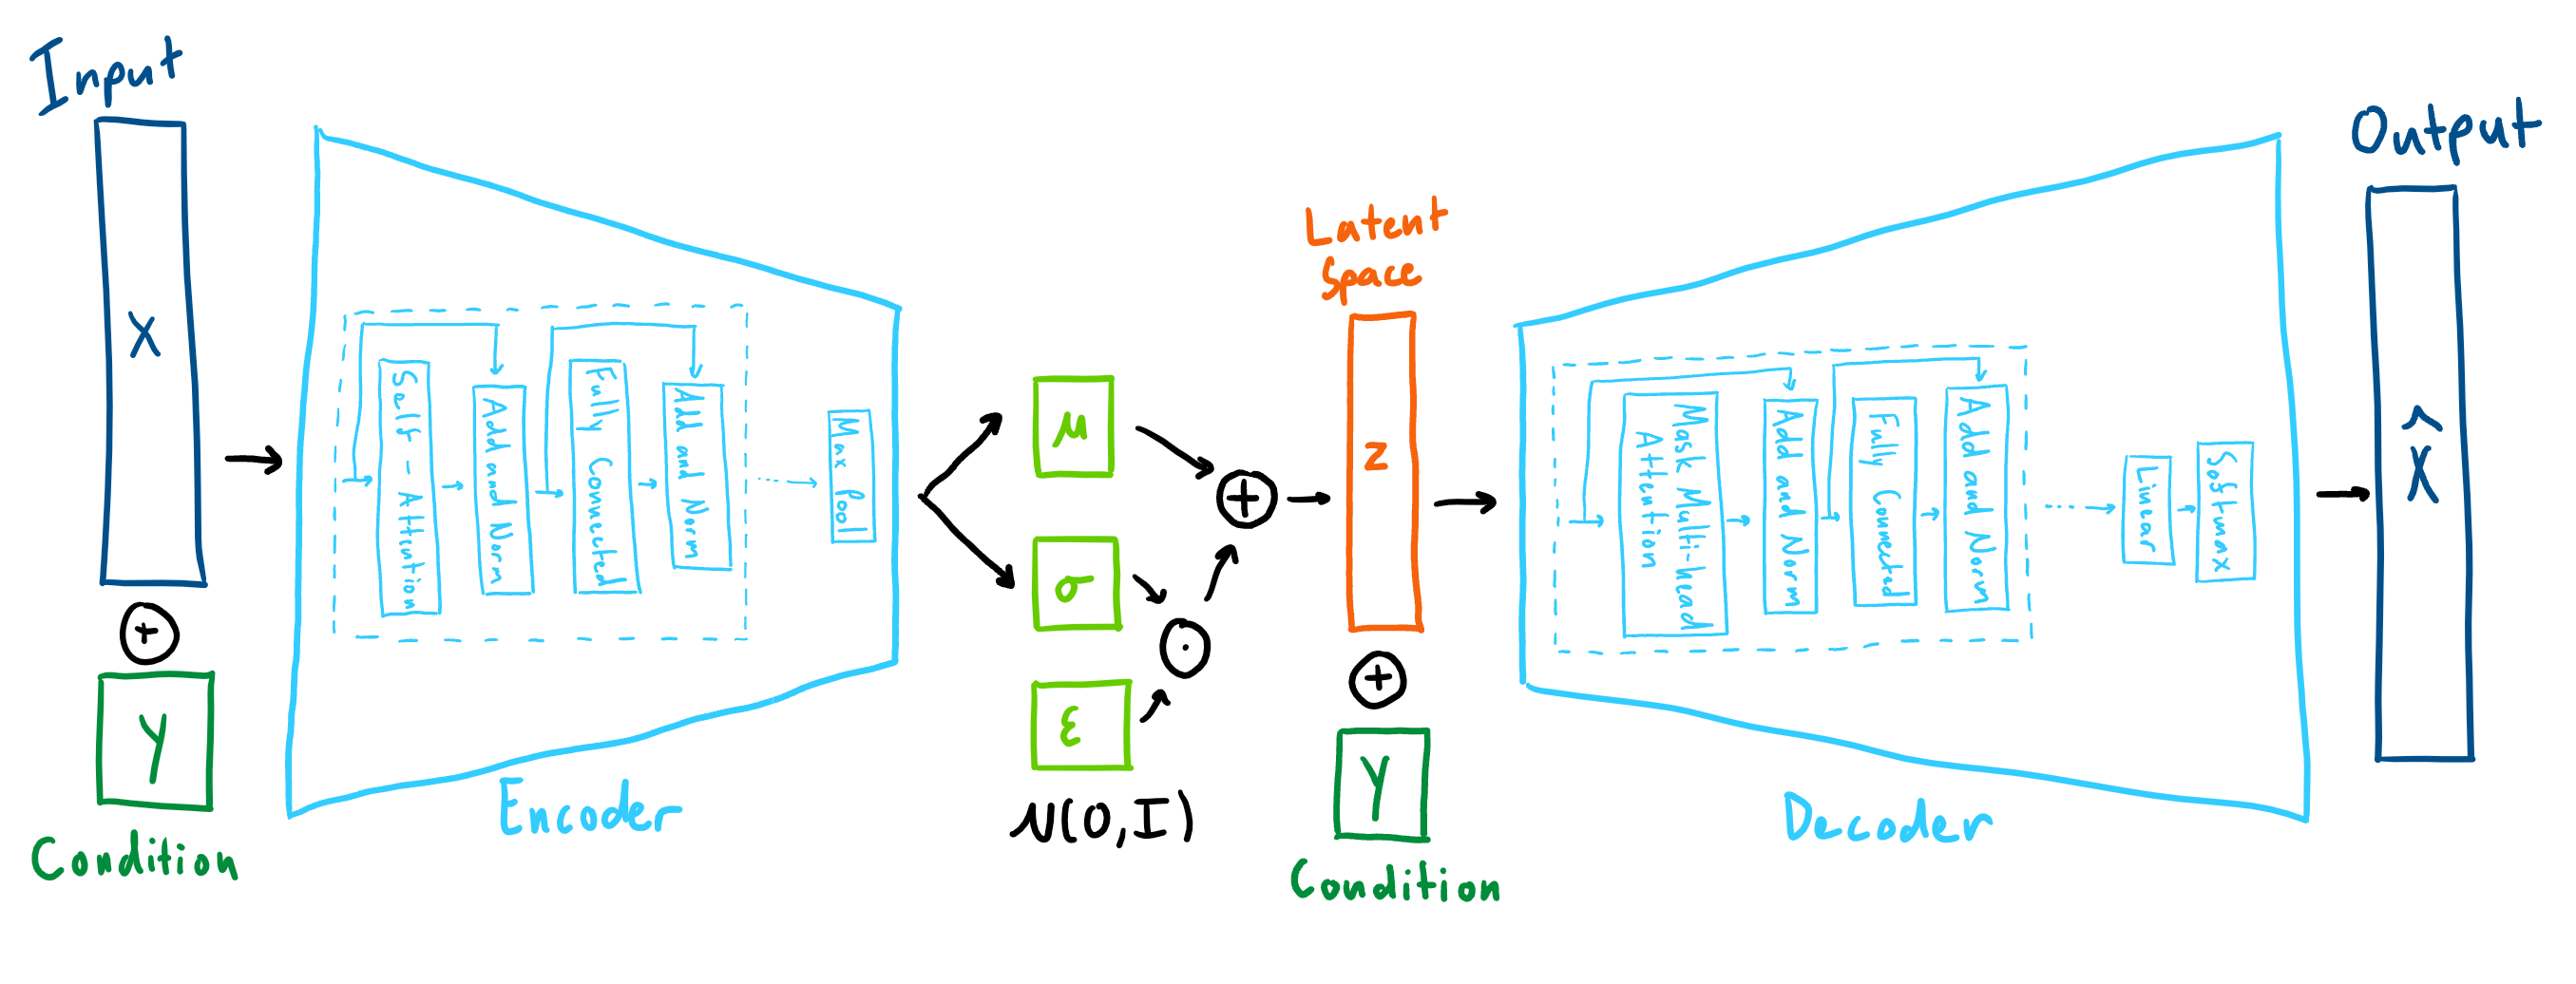
\includegraphics[width=\linewidth]{Pictures/CVAE_Architecture.png} 
    \end{minipage}
    \caption{Conditional Variational Autoencoder with Transformer Architecture} 
\end{figure}


\subsection{Advantages}
Our CVAE gRNA generator offers notable advantages. Namely, the transformer-based architecture can learn more long range dependencies and complex, data-driven patterns from sequential data using self-attention. This is particularly valuable for assessing nonlinear relationships between the biological factors that influence gRNA efficiency, which are defined in section 2 and are generally difficult for a researcher to experimentally test and validate \hyperref[Reference 6]{[6]}\hyperref[Reference 8]{[8]}\hyperref[Reference 11]{[11]}. Transformers enable all tokens in an input sequence to interact simultaneously and can reduce the probability of information loss in long DNA sequences \hyperref[Reference 13]{[13]}.

Furthermore, the use of positional encoding facilitates smooth gradient flow for backpropagation and optimization. The inherent periodicity of sine and cosine functions allows the model to encode and learn patterns, even at far-away positions, as they recur every period.  As a result, the model doesn't require sequential tracking of tokens like RNNs do. Instead, attention can infer relative distances between tokens through linear transformations and dot product similarity to learn sequential patterns in a parallel manner without explicit recurrence and generalize to unseen sequences. This is critical for our task, in which the order of DNA bases across a sequence carries significant information \hyperref[Reference 13]{[13]}. This generates contextually-rich gRNA sequences conditioned on target sequences and the learned latent space. The learned latent space captures the semantic information between DNA sequences and their effective gRNA counterparts, which allows the model to map novel DNA sequences to corresponding optimal gRNA sequences.

Additionally, the human genome has $6\cdot10^8$ potential gRNA sequences with NGG PAM, meaning that many existing heuristic-based and traditional generator models account for less than 0.01\% of all possible cases \hyperref[Reference 15]{[15]}. This means a high percentage of potential gRNA sequences have never been explored and tested. This allows for researchers to have a better baseline to narrow down unique gRNA sequences that heuristic generators may not produce and study novel gRNA sequences.


\subsection{Limitations}
Many biological factors are based on complex systems and processes that cannot be fully modeled without knowing the underlying factors which may not be fully captured by even the most sophisticated machine learning models. 

Some of these limitations include the scoring data we are using is measuring on-site efficiency and not considering off-site efficiency. This means it measures the performance of the gRNA in finding its target DNA and binding but fails to consider how often it binds to similar looking, but off-target sites. This is somewhere you would want to be more conservative with because having a very high-efficient gRNA can either mean you have a very precise gRNA that finds only its target DNA or it could mean you have a very indiscriminate gRNA that binds to anything remotely similar to your target DNA. This could be problematic especially in gene therapy where gene cuts or substitutions need to be done only at specific spots and off-target sites may alter another gene. 

High accuracy for matching to DNA is very important so we cannot only rely on efficiency scores for novel gRNA and target DNA pairs because mismatches can ``lead to off-target effects, depending on the number of mismatches and their positions.'' \hyperref[Reference 14]{[14]} This highlights the importance of our gRNA generator as a guiding design tool for gRNA to be then lab tested, not a substitution for rule-based design.

Another limitation with our approach is that we are not adding any specific design rules that may add bias towards certain heuristics and infer incorrect heuristics that disagree with existing design rules. There is always the possibility that machine learning models can disprove existing heursitic paradigms and discover new design rules. Nevertheless, incorporating well-established, deterministic rules into our deep-learning model such as the ratio of nucleotides, G and C, needing to be at 40-80\% to ensure gRNA stability, would leave less up to chance given that our approach relies on the model learning these rules on its own \hyperref[Reference 14]{[14]}. Our current proposed solution relies purely on the self-attention in the transformer to learn the rules and establish more complex relationships. With more research and resources, we could potentially make an improved transformer based model that incorporates known gRNA design rules crossed referenced with learned design rules to create more accurate gRNA generation.




\newpage

\section*{References}

\small
\label{Reference 1} [1] Anthon, Christian et al. “CRISPRon/off: CRISPR/Cas9 on- and off-target gRNA design.” Bioinformatics (Oxford, England) vol. 38,24 (2022): 5437-5439. doi:10.1093/bioinformatics/btac697 

\label{Reference 2} [2] Baisya, D., Ramesh, A., Schwartz, C. et al. Genome-wide functional screens enable the prediction of high activity CRISPR-Cas9 and -Cas12a guides in Yarrowia lipolytica. Nat Commun 13, 922 (2022). https://doi.org/10.1038/s41467-022-28540-0

\label{Reference 3} [3] Chuai, G., Ma, H., Yan, J. et al. DeepCRISPR: optimized CRISPR guide RNA design by deep learning. Genome Biol 19, 80 (2018). https://doi.org/10.1186/s13059-018-1459-4

\label{Reference 4} [4] Haeussler, M., Schönig, K., Eckert, H. et al. Evaluation of off-target and on-target scoring algorithms and integration into the guide RNA selection tool CRISPOR. Genome Biol 17, 148 (2016). https://doi.org/10.1186/s13059-016-1012-2

\label{Reference 5} [5] Jinek, Martin et al. “A programmable dual-RNA-guided DNA endonuclease in adaptive bacterial immunity.” Science (New York, N.Y.) vol. 337,6096 (2012): 816-21. doi:10.1126/science.1225829

\label{Reference 6} [6] Kornel Labun, Tessa G Montague, Maximilian Krause, Yamila N Torres Cleuren, Håkon Tjeldnes, Eivind Valen, CHOPCHOP v3: expanding the CRISPR web toolbox beyond genome editing, Nucleic Acids Research, Volume 47, Issue W1, 02 July 2019, Pages W171–W174, https://doi.org/10.1093/nar/gkz365

\label{Reference 7} [7] Xiang, X., Corsi, G.I., Anthon, C. et al. Enhancing CRISPR-Cas9 gRNA efficiency prediction by data integration and deep learning. Nat Commun 12, 3238 (2021). https://doi.org/10.1038/s41467-021-23576-0

\label{Reference 8} [8] Xu H, Xiao T, Chen CH, Li W, Meyer CA, Wu Q, Wu D, Cong L, Zhang F, Liu JS, Brown M, Liu XS. Sequence determinants of improved CRISPR sgRNA design. Genome Res. 2015 Aug;25(8):1147-57. doi: 10.1101/gr.191452.115. Epub 2015 Jun 10. PMID: 26063738; PMCID: PMC4509999. 

\label{Reference 9} [9] Attention Is All You Need, Ashish Vaswani and Noam Shazeer and Niki Parmar and Jakob Uszkoreit and Llion Jones and Aidan N. Gomez and Lukasz Kaiser and Illia Polosukhin, 2023, 1706.03762, arXiv, cs.CL, https://arxiv.org/abs/1706.03762

\label{Reference 10} [10] CRISPR Cas9 Image, https://www.elveflow.com/microfluidic-reviews/crispr-cas9-and-its-relation-with-microfluidics/

\label{Reference 11} [11] Mingkun Luo, Jun Wang, Zaijie Dong, Chenghui Wang, Guoqing Lu, CRISPR-Cas9 sgRNA design and outcome assessment: Bioinformatics tools and aquaculture applications, Aquaculture and Fisheries, Volume 7, Issue 2, 2022, Pages 121-130, ISSN 2468-550X, https://doi.org/10.1016/j.aaf.2021.10.002.

\label{Reference 12} [12] Kingma DP, Welling M. Auto-Encoding Variational Bayes. arXiv [stat.ML]. 2013 Dec 20. Available from: https://arxiv.org/abs/1312.6114. doi: 10.48550/arXiv.1312.6114.

\label{Reference 13} [13] Choi SR, Lee M. Transformer Architecture and Attention Mechanisms in Genome Data Analysis: A Comprehensive Review. Biology (Basel). 2023 Jul 22;12(7):1033. doi: 10.3390/biology12071033. PMID: 37508462;

\label{Reference 14} [14] Synthego. “How to Design Your Single Guide RNA (sgRNA).” \textit{Synthego}, https://www.synthego.com/guide/how-to-use-crispr/sgrna. Accessed May 13, 2025.

\label{Reference 15} [15] Zhang, H., Yan, J., Lu, Z. et al. “Deep sampling of gRNA in the human genome and deep-learning-informed prediction of gRNA activities.” \textit{Cell Discovery}, vol. 9, 48 (2023). https://doi.org/10.1038/s41421-023-00549-9

\label{Reference 16} [16] Liang Y. Variational Autoencoders. ECE 285 Deep Generative Models - Guest Lecture, 2024.


\end{document}